\documentclass[runningheads]{llncs}
\usepackage[T1]{fontenc}
\usepackage{graphicx}
\usepackage{amsmath}
\usepackage{amssymb}
\usepackage{multirow}
\usepackage{url}
\usepackage[spanish,es-tabla]{babel}

\begin{document}
\title{TLA+}
\author{Anna Aimeri, Sebastián Giraudo, Valentín Negrelli}
\institute{Facultad de Matemática, Astronomía, Física y Computación, Av. Medina Allende s/n, Córdoba, Argentina}
\maketitle              % typeset the header of the contribution
%
\begin{abstract}
Se presenta un set de herramientas sobre el lenguaje de especificación de modelos TLA+, que permite corregir el diseño de un sistema mediante la especificación de un modelo, y demostrar propiedades sobre sus comportamientos posibles mediante el uso de motores de prueba sobre lógica temporal de acciones. Se desarrollan características de la interfaz de usuario, el mecanismo de chequeo del modelo y especificaciones,  y casos de aplicación en la industria por grandes tecnológicas, desde procesos de sistemas operativos en tiempo real hasta sistemas de almacenamiento distribuidos.
\end{abstract}

\section{Introducción}
La complejidad de un sistema tiene incidencia directa en la probabilidad de agregar errores en el diseño y codificación del sistema a implementar, los cuales pueden derivar en pérdida o corrupción de la información, así como en violación de contratos con interfaces externas. Es así como la necesidad de tener un nivel de confianza máximo en el comportamiento en tiempo real del sistema se vuelve de vital importancia, haciendo necesarias pero insuficientes las técnicas de verificación de software estándar, tales como revisiones de código, testing de diseño, análisis de código estático, testing por estrés, por inyección de fallas, entre otros. 

Es en este contexto que surgen el chequeo de modelado y las pruebas sobre especificaciones como recursos útiles para medir corrección, completitud, progreso, y otras características deseables de un sistema, al analizar automáticamente todas las ejecuciones posibles de un sistema complejo.

En el presente trabajo se desarrollarán las herramientas de verificación sobre el lenguaje de especificación TLA+ (Temporal Logic of Actions), en particular del model-checker TLC y el sistema de pruebas TLA+ Proof System, sus objetivos, los aspectos técnicos de su funcionamiento, y casos de estudio que utilizaron estas herramientas en la industria junto con los resultados que arrojaron.


\section{Contexto de creación}

\section{Objetivo}
TLA+ es un lenguaje de especificación formal multi-propósito particularmente útil para describir sistemas distribuidos y concurrentes. Se trata de un lenguaje declarativo, jerárquico, y escalable a especificaciones de grandes sistemas, que provee una abstracción consistente sobre varios motores de prueba como backend. 

Las propiedades que TLA+ puede chequear son condiciones sobre ejecuciones individuales. Además permite verificar invariantes sobre comportamientos válidos tales como algunas propiedades de lógica temporal básica que respondan a características de safety y liveness, pudiendo asumir condiciones como fairness débil o fuerte sobre acciones.

Dado que el objetivo de la herramienta es especificar propiedades sobre las variables libres del modelo, es utilizado principalmente en la etapa de arquitectura y diseño del software, una vez que se cuenta con la especificación y antes de codificar la implementación. A su vez, es posible apoyarse en la herramienta para derivar casos de tests, dado que un diseño certero del modelo nos provee el conjunto de propiedades a verificar para nuestra implementación.

\section{Descripción del lado del usuario}
El entorno de desarrollo integrado (IDE) para las herramientas de TLA+ es TLA Toolbox, y puede utilizarse para diseñar las especificaciones, correr el model checker (TLC) y el TLA Proof System (TLAPS) \cite{tla}. Además, es posible correr el model checker vía línea de comandos \cite{book} o a través de una extensión para Visual Studio Code, que cuenta con las funcionalidades básicas del IDE.

El lenguaje de especificación de modelos TLA+ es un lenguaje formal que combina la lógica matemática con la teoría de conjuntos. Las especificaciones se disponen en módulos que describen el comportamiento global del sistema, expresando propiedades que deben mantenerse a lo largo del tiempo. Estos módulos contienen variables que representan los estados del sistema, descritos mediante expresiones lógicas. Además, pueden contener constantes, definiciones de operadores, teoremas y aseveraciones. En el contexto del lenguaje, las acciones describen las transiciones entre estados, y se definen con expresiones lógicas que relacionan el estado actual con su sucesor.

El lenguaje de propiedades de TLA+ se basa en la lógica de acciones temporales (TLA). Esta lógica combina la lógica temporal con una lógica de acciones, proporcionando constructores que incluyen predicados sobre estados iniciales, relaciones de transición entre estados sucesivos y condiciones de fairness para garantizar un progreso adecuado en el sistema.

TLA+ permite realizar un análisis exhaustivo de propiedades críticas, como la detección de deadlocks, y el análisis de progreso, garantizando que el sistema avance hacia estados deseados. Además, TLA+ facilita la verificación de invariantes, propiedades que deben mantenerse verdaderas en todos los estados alcanzables del sistema, a través de fórmulas especificadas en los archivos de configuración. También permite el control de fairness, mediante la conjunción de fórmulas temporales que definen las condiciones de liveness del sistema. (\textbf{EJEMPLO: esquema basico de especificacion en TLA}). Los análisis se realizan evaluando predicados de estado inicial y acciones de siguiente estado especificadas, utilizando evaluaciones para eliminar posibles transiciones o estados, garantizando una revisión completa y precisa del comportamiento del sistema bajo diferentes condiciones. 

Además, es posible con TLA+ formular teoremas y diseñar pruebas formales sobre propiedades de estas especificaciones en TLAPS. (\textbf{AGREGAR MAS SOBRE TLAPS)}

Los modelos en TLA+ y su verificación en TLC ponen su foco en el comportamiento del sistema, abstrayéndose de los detalles de su implementación. Es por esto que son independientes de cualquier lenguaje de programación, y no es necesario anotar el programa. Sin embargo, es posible anotar el algoritmo usando el pseudo-código PlusCal, un lenguaje formal que se transpila a TLA+, para probar propiedades sobre sus variables. A diferencia del enfoque orientado a acciones, PlusCal se asemeja más a un lenguaje de programación imperativo y es más adecuado para especificar algoritmos secuenciales. (\textbf{EJEMPLO: snippet en PlusCal}).

TLC visualiza los errores en las especificaciones de TLA+ proporcionando informes detallados cuando encuentra la violación de alguna propiedad. Cuando TLC detecta que una de las propiedades que está verificando no se cumple, procede a reportar un contraejemplo que ilustra cómo el sistema llega a un estado en el que esa propiedad es violada, a partir de un comportamiento válido segun la especificación. A continuación, TLC genera una traza que lleva al estado donde se produce la violación, representando cada estado como un predicado TLA+ que describe sus condiciones, y permite visualizar la evolución del sistema hasta llegar al estado problemático. Esta traza se minimiza para ofrecer una representación concisa pero informativa del problema. 

Los errores más difíciles de localizar son aquellos que TLC detecta al evaluar una expresión que no puede manejar o que produce un resultado no válido según la semántica de TLA+. TLC imprime la ubicación del error, indicando las expresiones anidadas que estaban siendo evaluadas cuando ocurrió el problema. A menudo, el reporte del error no es tan específico como se desearía, por lo que a veces es necesario insertar expresiones de impresión adicionales para localizar el problema con mayor precisión.

El verificador de modelos TLC permite la simulación de comportamientos del sistema. En modo de simulación, TLC construye y verifica repetidamente comportamientos individuales con una longitud máxima fija.

% opinion seba: a este parrafo capaz lo sacaría lpm
% como que ya nos metemos con como funciona por detras creo no? no tanto la UI
% capaz mergearlo con el primero y/o segundo de asp tecnicos
Para crear y verificar un comportamiento, TLC sigue un procedimiento similar al de construir el grafo G (\textbf{CUIDADO:} Acá hablamos del “grafo g” antes de definirlo), pero con una diferencia clave; después de calcular el conjunto de estados iniciales y el conjunto de sucesores para un estado dado, TLC elige pseudo-aleatoriamente un elemento de ese conjunto. Si el elemento no cumple con la restricción especificada, TLC detiene la computación de G. De lo contrario, TLC incluye ese estado en G y verifica las fórmulas de invarianza para ese estado. La construcción de G se detiene cuando se genera el número máximo especificado de estados.

\section{Aspectos técnicos}
TLC representa el espacio de estado de manera explícita utilizando un grafo dirigido G cuyos nodos son los estados del sistema. Este grafo es una parte del grafo de alcanzabilidad del estado que TLC ha encontrado hasta el momento. Además, TLC mantiene una cola U de estados que aún no han sido visitados o cuyos sucesores aún no han sido calculados.

El model checker utiliza Breadth First Search para explorar los estados alcanzables de un sistema y verificar que cumplen con las invariantes especificadas. Comienza evaluando los supuestos y calculando los estados iniciales. A partir de estos estados, TLC los añade a una cola y un grafo si cumplen con las restricciones iniciales. Este método garantiza que todos los estados alcanzables se examinen sistemáticamente. Si TLC encuentra un estado sin sucesores posibles reporta un estado de deadlock, indicando que el sistema no puede progresar más desde ese punto.

TLC no considera todo el espacio de estado, sino una parte de él. Utiliza una técnica de exploración exhaustiva, pero debido a limitaciones computacionales, de tiempo y de memoria, no es posible examinar todos los posibles estados de un sistema. En su lugar, TLC emplea estrategias inteligentes para explorar una porción representativa y significativa del espacio de estados, con el objetivo de detectar posibles problemas o violaciones de propiedades específicas en el modelo. Estas estrategias incluyen la generación de estados de manera incremental, el uso de técnicas de reducción como la simetría, y la exploración de estados que sean relevantes para las propiedades que se están verificando. De esta manera, TLC busca equilibrar la exhaustividad de la verificación con la eficiencia computacional, permitiendo obtener resultados significativos en un tiempo razonable.

En el contexto de TLA+, la simetría se aprovecha para reducir el número de estados que TLC necesita examinar al verificar una especificación. Si una especificación es simétrica con respecto a una permutación $\pi$, esto significa que si una secuencia de estados $\sigma$ satisface la especificación, entonces cualquier permutación de esa secuencia, $\sigma\pi$, también lo hará. Por lo tanto, si TLC ya ha verificado un comportamiento $\sigma$, no necesita verificar cualquier $\sigma\pi$ correspondiente, ya que cualquier error revelado por $\sigma$ también se revelaría por $\sigma\pi$.
Para aprovechar esta simetría, se puede incluir una declaración SYMMETRY en el archivo de configuración de TLC, definiendo un conjunto de permutaciones relevantes. Esto permite a TLC evitar agregar estados redundantes a su cola de estados no examinados y al grafo de estados si esos estados ya existen bajo alguna permutación.

En TLA+, se puede escribir una especificación de un programa que implementa una especificación más general mediante un mapeo de refinamiento adecuado. Este proceso implica mapear las variables de la especificación que se desea que el programa satisfaga con los estados de la especificación del programa en cuestión. El mapeo de refinamiento explica detalladamente cómo el programa cumple con la especificación general, lo que permite abstraer detalles específicos del programa y centrarse en su comportamiento general, asegurando que se cumplan las propiedades deseadas a nivel de especificación más alta.

\textbf{(FALTA RESPUESTA)}

En la verificación de modelos con TLC es posible que se generen falsos negativos, especialmente en el contexto de propiedades de liveness. Esto se debe a la dificultad de detectar violaciones de propiedades de liveness con modelos finitos, ya que estas propiedades requieren que el sistema alcance ciertos estados infinitas veces o en un orden específico, lo cual puede ser imposible de capturar con un modelo de estas características.

\textbf{(FALTA TLAPS)}

\section{Casos de estudio}
\subsection{Intel}
En Intel, TLA+ y TLC se han utilizado para diseñar y verificar protocolos de coherencia de caché en procesadores multinúcleo, en particular para los procesadores Alpha EV7 y EV8. En particular para el proyecto del EV8, la especificación fue completada antes de que el diseño fuera estable, lo que brindó feedback a los diseñadores.

TLA+ facilita la exploración de optimizaciones y modificaciones del protocolo, permitiendo iteraciones rápidas y evaluaciones de su impacto en la complejidad del estado. La experiencia de los ingenieros de Intel muestra que TLA+ es una herramienta poderosa para encontrar errores y mejorar la eficiencia de los diseños complejos en etapas tempranas del desarrollo. \cite{tla}

\subsection{Amazon}
TLA+ se utilizó en Amazon Web Services (AWS) \cite{amazon} para corregir errores y mejorar la fiabilidad del sistema mediante especificación formal y verificación de modelos. En este caso, un desarrollador utilizó TLA+ para abordar un error sutil en un algoritmo que había pasado desapercibido a través de múltiples revisiones de diseño y código. A pesar de meses de pruebas, el error surgió sólo después de que el desarrollador escribiera una especificación en TLA+ y la ejecutara en el verificador de modelos TLC, que identificó rápidamente el problema. Esta detección exitosa de errores destacó la efectividad de TLA+ para descubrir defectos ocultos que los métodos de prueba tradicionales podrían pasar por alto.

% Amigos miren como separe el propiedades para forzar un salto de línea
% es horrible pero no se por que se buggea y no salta automaticamente
La fortaleza de TLA+ radica en su capacidad para describir tanto las propie-\\dades de corrección deseadas del sistema (el 'qué') como el diseño del sistema (el 'cómo'). Esto permite a los desarrolladores no solo verificar la corrección del sistema, sino también comprender su funcionamiento interno y realizar optimizaciones de rendimiento sin sacrificar la corrección. Debido al gran volumen de procesos que se realizan en los servidores de AWS, garantizar un código con la menor cantidad de bugs posible es esencial. Aunque un bug pueda parecer poco probable y tener una probabilidad de ocurrencia muy baja, la enorme cantidad de transacciones que se realizan diariamente hace que incluso estos casos poco probables puedan surgir. Por lo tanto, la capacidad de TLA+ para detectar y corregir incluso los errores más sutiles se vuelve crítica en un entorno donde la fiabilidad y la precisión son imperativas.

Además, el éxito del uso de TLA+ para rectificar errores llevó a la dirección de AWS a abogar por su adopción en otros equipos que trabajaban en algoritmos y características críticas dentro del servicio S3. Los desarrolladores escribieron especificaciones formales para algoritmos adicionales y nuevas características, con el verificador de modelos ayudando a verificar las correcciones y prevenir la introducción de nuevos errores. La capacidad de enseñar rápidamente TLA+ a desarrolladores nuevos en la herramienta fue crucial para escalar su adopción dentro de la organización, demostrando su valor en mejorar la calidad del sistema y prevenir que errores graves lleguen a producción.

En la Tabla \ref{tab1} obtenida del paper podemos ver en qué sistemas dentro de AWS fue usado TLA+, y cómo le fue beneficioso.

\begin{table}
    \caption{Aplicaciones de TLA+ en Amazon.}\label{tab1}
    \setlength{\tabcolsep}{2pt} % Adjust column separation
    \begin{tabular}{|p{4.5em}|p{11em}|p{6em}|p{15em}|}
    \hline
    Sistema & Componentes & Cantidad de líneas & Beneficio\\
    \hline
    \multirow{2}{*}{S3} & Fault-tolerant low-level network algorithm & 804 PlusCal & Found 2 bugs. Found further bugs in proposed optimizations.\\
    \cline{2-4}
     & Background redistribution of data & 645 PlusCal & Found 1 bug, and found a bug in the first proposed fix.\\
    \hline
    \parbox{4em}{Dynamo DB} & Replication \& group & 939 TLA+ & Found 3 bugs, some requiring traces of 35 steps\\
    \hline
    EBS & Volume management & 102 PlusCal & Found 3 bugs.\\
    \hline
    \multirow{2}{*}{\parbox{4em}{Internal distributed\\lock manager}} & Lock-free data structure & 223 PlusCal & Improved confidence. Failed to find a liveness bug as we did not check liveness.\\
    \cline{2-4}
     & Fault tolerant replication and reconfiguration algorithm & 318 TLA+ & Found 1 bug. Verified an aggressive optimization. \\
    \hline
    \end{tabular}
\end{table}
 
\subsection{Elasticsearch}
En la versión 6.2 de ElasticSearch se detectó un bug \cite{elastic_search} que dejaba documentos borrados sin eliminar accesibles si se tenía acceso seguro, un valor booleano compartido, al momento de la operación, y el sistema de mapeo de versiones era vulnerable a cambios en este valor que permitía leer el documento eliminado. De modo que fueron reportados casos por usuarios que encontraron documentos con la misma clave primaria, tras hacer llamadas a sus APIs de indexación y eliminación de documentos consecutivamente. 

Estos casos fueron detectados por TLC en un modelo formal realizado por los propios desarrolladores del sistema de indexación y eliminación de documentos replicados. Pudieron solucionar el problema eliminando estos documentos cuando hayan sido re-indexados, sin importar la condición del valor de acceso seguro. Con esto pudieron pasar las pruebas de TLC sobre terminación del proceso

\begin{equation}
    Terminated \triangleq \forall self \in ProcSet: pc[self] = "Done"
\end{equation}

Y el invariante de unicidad de documentos
% \begin{align*}
%     & Invariant \triangleq Terminated \implies \\
%     & \land expected\_doc = NULL \implies lucene\_document = NULL \\ 
%     & \land expected\_doc \neq NULL \implies lucene\_document.content = expected\_doc
% \end{align*}
% Dejo esto que me compiló en overleaf pero no tengo el compilador asi que comentado
% esta como estaba antes jiij
\[
\begin{aligned}
    &Invariant \triangleq Terminated \implies \\
    &\phantom{Inv} \land expected\_doc = NULL \implies lucene\_document = NULL \\ 
    &\phantom{Inv} \land expected\_doc \neq NULL \implies lucene\_document.content = expected\_doc
\end{aligned}
\]


\subsection{Prueba de un algoritmo tolerante a demoras y fallas de renombre de procesos}
En el marco de la computación paralela, se ha realizado un trabajo \cite{case_study} de análisis y verificación de un algoritmo no bloqueante y tolerante a fallas de renombre de procesos en un sistema de memoria compartido. Esto permite probar propiedades de safety y liveness sobre el sistema. En particular se probó la siguiente propiedad de corrección, 
\begin{equation}
    \forall p, q \in Proc, p \neq q, \square(name_p \neq \bot \land name_q \neq \bot \implies name_p \neq name_q)
\end{equation}

que cada proceso obtiene un nombre único, y la siguiente propiedad de terminación,
\begin{equation}
    \forall p \in Proc, \square(\text{p enters the renaming} \implies \lozenge (\text{name}_p \neq \bot))
\end{equation}

que cada proceso que entra al sistema obtiene un nombre.
Además se proveen las pruebas pertinentes de corrección y completitud de los splitters, objetos que se utilizan para la sincronización de acciones sin bloqueo,  las cuales son

\[
\square \left( \begin{aligned}
    &\phantom{\land} \forall p,q \in \text{Proc}, \phantom{\land} \text{dir}_p = \text{stop} \land \text{dir}_q = \text{stop} \implies p = q \\
    &\land \exists p \in \text{Proc}, \text{dir}_p \neq \text{right} \\
    &\land \exists p \in \text{Proc}, \text{dir}_p \neq \text{down}
\end{aligned} \right)
\]
y

\[
    \forall p \in Proc, \square(p\ entra\ al\ splitter \implies \lozenge(dir_p \in \{stop, down, right\})))    
\]

respectivamente.
El modelo y prueba de estas propiedades consisten en 2000 líneas de TLAPS para el algoritmo, y 200 líneas por el splitter, con un total de 70 lemas y teoremas, y 963 pasos de prueba. Las pruebas del splitter consisten en 93 obligaciones de prueba, entre ellas 43 obvias y descartadas por TLAPM (el manejador de pruebas de TLA+), y las otras 50 resueltas con motores de prueba SMT (CVC3, VeriT y Z3 fueron usados).

\section{Caso de aplicación de la herramienta}
A continuación desarrollamos un caso de aplicación completo donde podemos ver cómo se utiliza TLA+ y su verificador TLC para encontrar un bug en un proceso concurrente real.

Se trata de un modelo de gestor de tareas, creado por el desarrollador Andreas Stührk para la empresa donde trabaja. El mismo debe mantener actualizado el estado de realización de los trabajos encomendados, y encargarse de la realización concurrente de las mismas. El sistema tenía un bug de consistencia en el supervisor de trabajos, y es que a veces no se percibía el cambio de ‘pendiente’ a ‘completo’ correctamente. Por lo que se desarrolló la especificación de las partes del sistema existente con TLA+, particularmente usando su lenguaje de pseudocódigo asociado PlusCal también, y fueron chequeadas invariantes de correctitud y progreso con TLC.

Cada trabajo consiste en la completitud de tareas independientes. El sistema consiste de un supervisor de progreso, que toma los mensajes de status de tareas de una cola FIFO conectada a las unidades de procesamiento y decide si el trabajo está completo, y guarda la información del progreso en nodos en una unidad de almacenamiento (Cassandra). Esta unidad implementa factores de replicación y niveles de consistencia para asegurar que los datos sean replicados y leídos de manera confiable entre múltiples nodos. En la figura 1 se puede ver un diagrama de la arquitectura del sistema. 

\begin{figure}[t]
    \caption{Arquitectura del sistema gestor de tareas.}\label{sistema}
    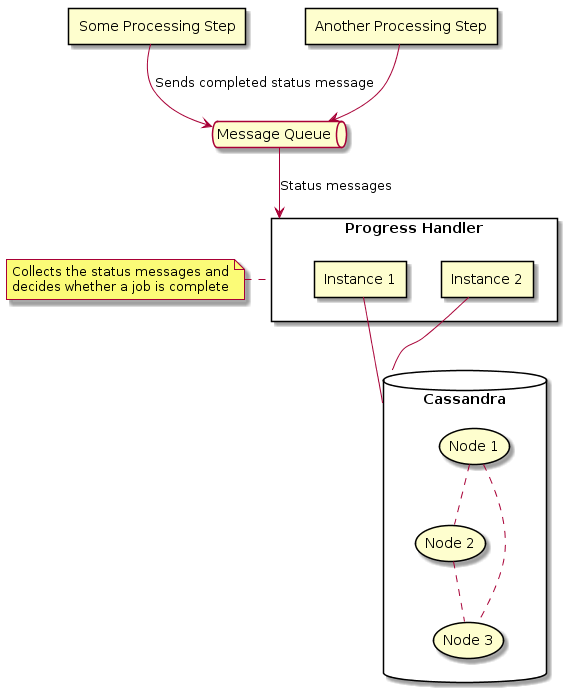
\includegraphics[width=8cm]{formalizing-the-system.png}
    \centering
\end{figure}


\begin{thebibliography}{8}
\bibitem{wiki}
Wikipedia, La Enciclopedia Libre, "TLA+", \url{https://en.wikipedia.org/wiki/TLA%2B}, último acceso 2024/05/28

\bibitem{tlaps}
TLA+ Proof System, \url{https://proofs.tlapl.us/doc/web/content/Home.html}, último acceso 2024/05/28

\bibitem{tla}
The TLA+ Home Page, \url{https://lamport.azurewebsites.net/tla/tla.html}, último acceso 2024/05/28

\bibitem{case_study}
Finding bugs in systems through formalization, \url{https://andy.hammerhartes.de/finding-bugs-in-systems-through-formalization.html}, último acceso 2024/05/28

\bibitem{amazon}
Chris N., Tim R., Fan Z., Bogdan M., Marc B., Michael D.: Use of Formal Methods at Amazon Web Services. Amazon.com, 29th September, 2014

\bibitem{elastic_search}
% NOTA: No sé bien cómo citar esto apropiadamente porque es un issue de github jajeji
Possible to index duplicate documents with same id and routing id, \url{https://github.com/elastic/elasticsearch/issues/31976#issuecomment-404722753}

\bibitem{book}
Leslie L.: Specifying Systems: The TLA+ Language and Tools for Hardware and Software Engineers. Addison-Wesley Professional, 2002

\end{thebibliography}
\end{document}
